\section{Path Conditions and the Abstraction Relation}
\label{sec:abstraction_relation}


This section will present how path conditions are structured to represent symbolic rule execution. As well, we define the abstraction relation between the execution of a DSLTrans transformation and the path condition that represents it.
This abstraction relation allows us to prove properties on a finite set of representative path conditions, as created by the path condition generation algorithm. As this set is finite, our technique is guaranteed to be decidable.


\subsection{Symbolic Execution}

Our algorithm operates on the principle of symbolic execution to build up these
path conditions. In order to explain the concept of symbolic execution of a
transformation, let us make an analogy with program symbolic execution as
introduced by King in his seminal work ``\emph{Symbolic Execution and Program
Testing}''~\cite{DBLP:journals/cacm/King76}. According to King, a symbolic
execution of a program is a set of \emph{constraints} on that program's
\emph{input variables} called \emph{path conditions}. Each \emph{path condition}
describes a traversal of the conditional branching commands of that program. A
\emph{path condition} is symbolic in the sense it \emph{abstracts} as many
concrete executions as there are instantiations of the path condition's
variables that render the path condition's constraints true.

We can transpose this notion of symbolic execution to model transformations. The
analog of an input variable in the model transformation context are
\emph{metamodel classes, relations and attributes}. As program statements impose
constraints on input and output variables during symbolic execution,
transformation rules impose conditions on which metamodel elements are
instantiated during a concrete transformation execution, and how that
instantiation happens. As well, rules in a model transformation are implicitly
or explicitly scheduled. These control and/or data dependencies must be
taken into consideration during path condition construction.

As in program symbolic execution, each path condition in our approach \emph{abstracts} as many concrete executions as there are input/output models
that satisfy them. This is formulated as an \emph{abstraction relation} as further explained in \cref{subsec:abstraction_relation}.

In what follows we will examine in more detail how these symbolic execution
principles can apply to the verification of model transformations.


\subsection{Path Conditions}
\label{sec:gen_path_conds}

In order to present the intuition of path conditions and symbolic executions, we
first discuss the idea of \textit{rule combinations}.

As seen in \cref{sec:dsltrans}, a layer in a DSLTrans transformation contains a
number of rules.  We can create a set of rule combinations for this layer by
taking the powerset of all rules in that layer. Each rule combination in this
set will represent all possible transformation executions where the rules in
that combination would execute.

For example, in \cref{fig:rule_combos2}, the rule combination marked `AC'
represents the set of transformation executions where the rules A and C would
execute and no others. Another rule combination marked `A' represents the
transformation executions where only rule A would execute.

\begin{figure}[h!] \centering 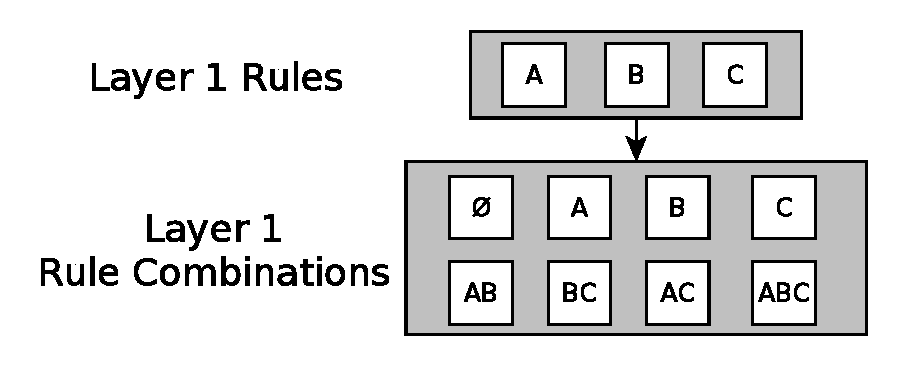
\includegraphics[width=.40\textwidth]{./figures/overview/rule_combos.pdf}
	\caption{Rule combinations created for a transformation layer}
	\label{fig:rule_combos2}
\end{figure}

Note that within these rule combinations, the number of times a rule has
executed is abstracted. Either a rule has executed zero times, and the rule is
not represented in a rule combination, or the rule has executed some finite
number of times and it is represented. This abstraction is key to our approach,
as it allows us to create a finite set of path conditions to abstract over an
infinite set of transformation executions, as seen in
\cref{subsec:abstraction_relation}.

We also note that rule \textit{combinations} are created, and not rule
\textit{permutations}. This follows from the semantics of \\DSLTrans as described
in \cref{sec:dsltrans}, as transformation rules in a layer will execute in a
non-deterministic order but produce a deterministic result, by construction of the semantics of DSLTrans. As a final
note, the transformation executions that these rule combinations represent always terminate, also by construction of the semantics of DSLTrans~\cite{DBLP:conf/sle/BarrocaLAFS10}.

We base our concept of path conditions on these rule combinations. However, as
DSLTrans allows for dependencies between rules, we cannot create path conditions
for the transformation by taking the powerset of all rules. Instead, our
approach must move layer-by-layer and resolve the dependencies between rules.
The next two sections will introduce the concepts of traceability and dependency, before we
briefly discuss the syntax and semantics of path conditions themselves.

\subsubsection{Traceability}
\label{subsubsec:traceability}

DSLTrans rules specify which elements of the
output model were created from specific elements of the input model. To resolve
these dependencies, traceability information for the transformation is created
during the execution of a DSLTrans model transformation~\cite{DBLP:conf/sle/BarrocaLAFS10}.
In our verification approach, we store this same information as symbolic \emph{traceability links}, in
order to record which elements belong to the same DSLTrans rule.


At a particular point in the path condition construction process, symbolic traceability links are built for
each rule as follows: for all match and apply elements of a rule, given a match
element belonging to the match graph of a rule and an apply element belonging to
the apply graph of the same rule, a symbolic traceability link is built between the two
if the apply element is not connected to a backward link (as explained below).
This is intuitive: traceability links are built between a newly generated
element in the output model, and the elements of the input model that originated
it.

\begin{figure}[htb]
        \centering
        \begin{subfigure}[b]{0.24\textwidth}
                \centering
                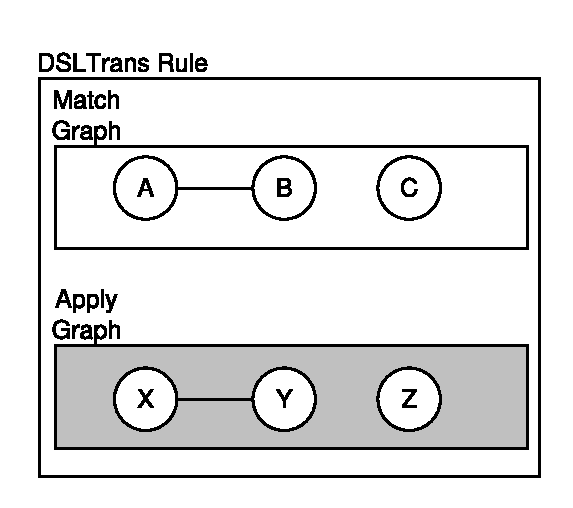
\includegraphics[width=1\textwidth]{./figures/building_path_conditions/traceability_links.pdf}
                \caption{Before symbolic traceability links added}
                \label{fig:traceability_links1}
        \end{subfigure}%
        ~~
        \begin{subfigure}[b]{0.235\textwidth}
                \centering
                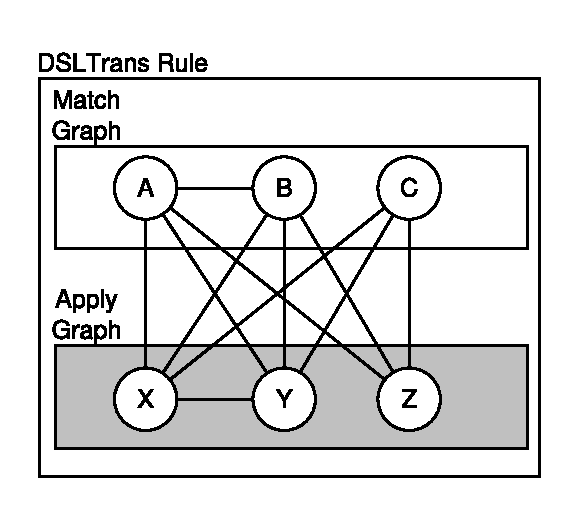
\includegraphics[width=1\textwidth]{./figures/building_path_conditions/traceability_links2.pdf}
                \caption{After symbolic traceability links added}
                \label{fig:traceability_links2}
        \end{subfigure}%
        \caption{Symbolic traceability links created for an abstract DSLTrans rule}
        \label{fig:trace_links}
\end{figure}

An example of the symbolic traceability link creation process is shown in
\cref{fig:trace_links}. Note that symbolic traceability links are solid lines between
match and apply elements in our visual notation.



\subsubsection{Backward Links}
\label{subsubsec:backward_links}

The dependencies in a DSLTrans rule are specified using the \textit{backward link} construct, as further detailed in \cref{subsec:DSLTrans_constructs} and \cref{def:transformation_rule}. \cref{subsubsec:resolve_dependencies} will discuss how these dependencies are then resolved during our symbolic execution approach.

\cref{fig:backward_links} demonstrates how backward links are used \\within a rule. The rule shown contains a backward link, which defines the dependency that an element of type X was created from an element of type A, and an element of type Y was created from an element of type B. If this dependency is satisfied, then another element of type Z should be created. This element should be associated with the Y element.

\begin{figure}[htb]
        \centering
        \begin{subfigure}[b]{0.235\textwidth}
                \centering
                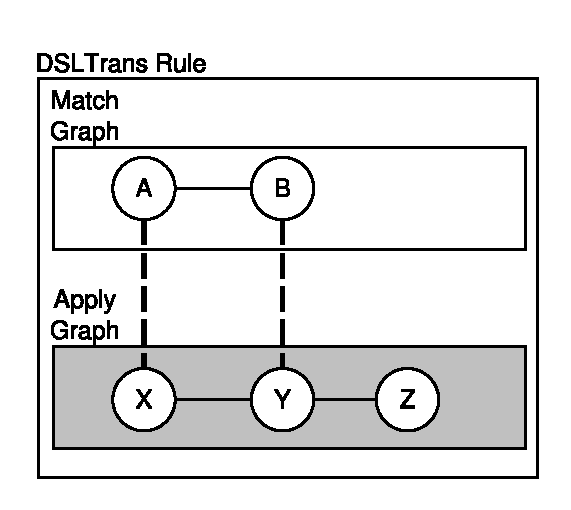
\includegraphics[width=1\textwidth]{./figures/building_path_conditions/backward_link.pdf}
                \caption{Rule with backward links (dashed lines)}
                \label{fig:backward_links}
        \end{subfigure}%
        ~~
        \begin{subfigure}[b]{0.235\textwidth}
                \centering
                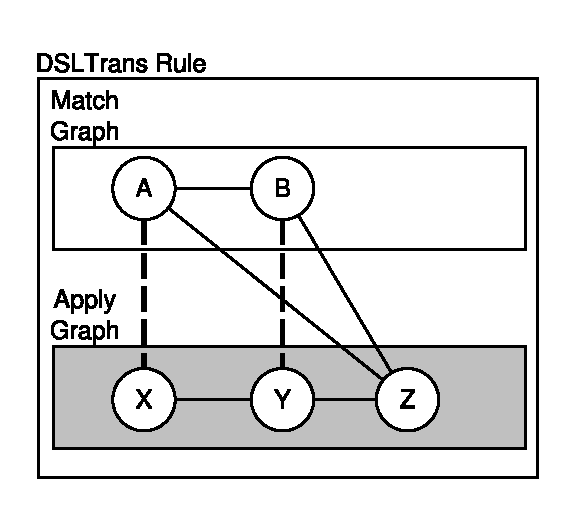
\includegraphics[width=1\textwidth]{./figures/building_path_conditions/backward_link2.pdf}
                \caption{Traceability links added\\~}
                \label{fig:backward_links2}
        \end{subfigure}%
        \caption{Adding traceability links to an abstract DSLTrans rule with backward links}
        \label{fig:back_links}
\end{figure}

\cref{fig:backward_links2} shows the rule after symbolic traceability links have been added. Two symbolic traceability links are created from the Z element to the A and B elements in the match graph to store traceability information. Note that no symbolic traceability links are built between two elements connected by backward links, as these links have already been built in a previous layer.



\subsubsection{Syntax and Semantics}
\label{subsubsec:path_condition_creation}

A path condition represents the symbolic execution of a set of DSLTrans rules, similar to a rule combination as explained above. Each path condition represents the execution of a set of transformation rules, by containing the input and output elements which are produced by the execution of those transformation rules.

Again, we use an abstraction over the number of times a rule has symbolically executed. Each path condition will represent that a rule has not executed, or has executed one or more times.

   \begin{figure}[t]
     \begin{center}
       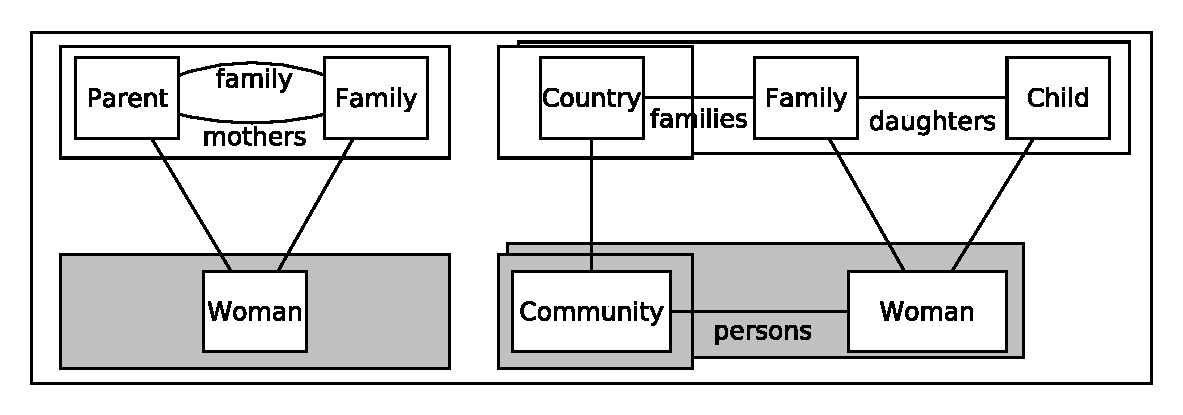
\includegraphics[width=0.45\textwidth]{figures/path_conditions/pc.pdf}
       \caption{An example path condition representing the execution of three rules}
       \label{fig:pc_first}
     \end{center}
     \vspace{-0.20in}
   \end{figure}
   
For example, the path condition in Figure~\ref{fig:pc_first} represents the execution of three rules in the transformation. This representation includes the input and output elements that will be present in the input and output models if these three rules execute. The set of path conditions produced by the prover will therefore partition the set of valid executions of the transformation, where each execution is an input/output model pair. This technique was first proposed in~\cite{Lucio2010} and further detailed in~\cite{Lucio2014}.


%The path condition generation algorithm will symbolically combine transformation rules into a path condition. Each path condition will then abstract a set of concrete transformation executions, as defined by our abstraction relation in \cref{sec:abstraction_relation}.



\begin{definition}{Path Condition\\}
\label{def:path_condition}

A path condition is a four-tuple $\big\langle \mathit{NAC}$, $\mathit{Input}$, $\mathit{Output}$, $\mathit{trace}\big\rangle$, where:

\begin{itemize}
\item $\mathit{NAC}, \mathit{Input}, \mathit{Output} \in \textsc{TG}$
\item $\mathit{Input}$ and $\mathit{Output} $ may be empty and are disjoint
\item $\mathit{NAC}$ may be an empty graph, and is disjoint from both $\mathit{Input}$ and $\mathit{Output} $
\item $\mathit{trace} = \{E_{trace}, (s_{trace}, t_{trace})\}$
\begin{itemize}
\item $E_{trace}$ contains the traceability links
\item $E_{trace} $ is disjoint from $E_{Input}$, $E_{Output}$, and $E_{NAC}$
\item $(s_{trace}, t_{trace})$ is a pair of functions $s_{trace}: E_{trace}\rightarrow V_{\textit{Output}}$ and $t_{trace}: E_{trace}\rightarrow V_{\textit{Input}}$ that respectively provide the source and target vertices for each traceability link
\end{itemize}

\end{itemize}  

The empty path condition is defined as $\{\emptyset, \emptyset, \emptyset, \emptyset \}$.

The set of all path conditions is noted as $\textsc{PathConds}$.

We also define a utility function getRules: PC $\rightarrow$ Set(Rules). This function accepts a path condition and returns the rules which were involved in its construction. This information will be used to report the status of contract proof. Note that operationally, this is done by storing the names of the rules within the path condition. 

We define a utility function getTransformation: PC $\rightarrow$ Transforms. This function returns the Transform that the path condition was built for. The purpose of this function is to restrict path condition to only be applicable for the transformation they represent.



\end{definition}



%\item Path conditions onto transformation executions
%\begin{itemize}
%\item Each rule in graph:
%\begin{itemize}
%\item As in paper. Match component is injectively found. Apply component is surjectively found.
%\item For traceability links, PC links are found injectively. Transformation executions links are found surjectively. Not a bijection because multiple rule executions could be present in transformation execution.
%
%\item Question: How to handle unification of matching. Seems to be straightforward before/after must match.
%\end{itemize}
%\end{itemize} 


The formal definition of a path condition is presented in \cref{def:path_condition}. Note that the structure of path conditions is intentionally very similar to that of DSLTrans rules and input-output models.

The \textit{input} graph of a path condition represents a pattern that must be present in the input model of the transformation, while the \textit{output} graph is a pattern which will be instantiated in the output model of the transformation. Symbolic traceability links are also kept between elements in the \textit{input} and \textit{output} graphs to retain traceability information.


Finally, we define a function getComponents: PC $\rightarrow$ Set(Typed Graph). This function is used for the abstraction relation, as it returns a set of subsets from the match graph of the path condition. These components are collections of the match graph of rules that have been overlaid on top of each other. These components must be matched as a unit, as their elements must be injectively matched. However, elements from different components may match onto the same target vertex in the abstraction relation. More information on how the components are constructed will be provided in the section on path condition construction. \bentley{This is not elegant at all...}



\subsection{Abstraction Relation}
\label{subsec:abstraction_relation}

Our abstraction relation is at the core of our technique. It allows us to represent an infinite set of transformation executions with a finite set of path conditions. As mentioned before, contract proof can then take place on this set of path conditions and hold on the set of transformation executions, as further explored in Section~\ref{sec:prop_satisfaction}.

Let us start by formally defining the notion of abstraction of a transformation
execution by a path condition.

LOOK AT COMPONENTS IN PC MATCH GRAPH AS ELEMENTS AND TRACE LINKS

THEN LOOK AT OUTPUT ELEMENTS AND TRACE LINKS IN IOM

REDO STRUCTURES TO ONLY BE ONE VERTEX AND EDGE SET, AND HAVE SUBSETS FOR MATCH, APPLY



\begin{definition}{Abstraction of a Transformation Execution by a Path Condition\\}
\label{def:abstraction_pc_ex}

Let $iom = \big\langle \mathit{Input}$, $\mathit{Output}$, $\mathit{trace}\big\rangle \in \textsc{IOM}$ be an input-output model, also known as a transformation execution. \bentley{Make sure this terminology is consistent.}

Let also $pc = \big\langle  \mathit{NAC}$, $\mathit{Input}$, $\mathit{Output}$, $\mathit{trace}\big\rangle  \in \textsc{PathConds}$ be a path condition.

We also require that getTransformation(iom) and getTransformation(pc) return the same transformation.

We have that $iom$ is abstracted by $pc$, noted $ex\Vvdash pc$, if and only if the following conditions are all true:


\noindent\makebox[\linewidth]{\rule{\linewidth}{0.4pt}}
The PC's NAC does not match onto the iom's Input

\begin{multline}
\label{eq:abstr_no_nac}
\nexists \big(\mathit{PC}_{NAC} \stackrel{inj}{\vartriangleleft} \mathit{iom}_{Input}^*\big)
\end{multline}

\noindent\makebox[\linewidth]{\rule{\linewidth}{0.4pt}}

Each component in the PC:
Elements matches on the iom's Input
Traceability links can be found as well

\begin{multline}
\label{eq:abstr_input_output}
\big(\forall \mathit{comp} \in \mathit{getComponents(PC)} \vartriangleleft Input^* : \mathit{comp} \stackrel{inj}{\vartriangleleft} \mathit{iom}_{Input}^*\big)
\end{multline}

\noindent\makebox[\linewidth]{\rule{\linewidth}{0.4pt}}

Elements in the iom's Output graph must surjectively match on the Output graph of the PC
Trace links in iom can be found in PC

\begin{multline}
\label{eq:abstr_apply_surjective_match}
\mathit{iom}_{Output} \stackrel{surj}{\vartriangleleft} \mathit{PC}_{Output}
\end{multline} 

\noindent\makebox[\linewidth]{\rule{\linewidth}{0.4pt}}

%\begin{multline}
%\label{eq:abstr_trace}
%
%\forall \mathit{PCTrace} \in \mathit{PC}_{trace} :
%
%\exists \mathit{IOMTrace} | \mathit{IOMTrace}
%
%\big(\forall trc\in Components(pc|_{trace})\;.\;trc\vartriangleleft ex\big)\;\land\;\\
%\big(\forall e'\in E'\, \exists e\in E\;.\;\tau'(e')=trace \Longrightarrow \tau(e)=trace\big)
%\end{multline} 
% where for all $rl,rl'\in Rules$, if $rl\cong rl'$ then there exist two injective typed graph homomorphisms $f$ and $g$ such that $Match(rl)\stackrel{f}{\vartriangleleft} Input^*$, $Match(rl)\stackrel{g}{\vartriangleleft} Input^*$ and $CoDom(f)\neq CoDom(g)$.
% $/pc/ = Apply_{ex}\cup ex|_{trace}$ is the output part of $pc$, including symbolic traceability links.

\reviewer{Definition 28: When you define the abstraction of an execution
  by a path condition, you require two conditions (separated by an
  and). I have the feeling that the morphisms used in both
  conditions should somehow be compatible to each other. However,
  your triangle notation indicates only the existence of a morphisms.
  How do you express that these morphisms somehow "agree"?}
  

  
  
\end{definition} 


% \cref{def:abstraction_pc_ex} enforces the fact that the matcher part of
% components of the path condition are found through an injective typed graph
% homomorphism in the execution's input model. Additionally, the graph including
% the output of the execution (including traceability information), can be
% mapped by a surjective typed graph homomorphism onto the apply model (plus the
% symbolic traceability links) of the path condition.

To understand the abstraction relation in \cref{def:abstraction_pc_ex}, recall
that during the construction of a transformation execution rules are matched
injectively in the input model. This information is present in the first
condition of the abstraction relation (Proposition~\ref{eq:abstr_input_output})
via the injective typed graph homomorphism between the match part of the copies
of rules ``glued'' onto the path condition and the containment transitive
closure of the input part of the transformation execution. This relation
enforces the fact that certain parts of the execution were found, or matched, by
certain parts of the path condition.
On the other hand, the surjection from the output of the execution towards the
apply part of the path condition models the fact that the output of the
execution has been completely built by instantiating the apply parts of the
rules contained in the path condition.

The second condition of the abstraction relation
(Proposition~\ref{eq:abstr_trace}) checks for the fact that symbolic
traceability links in the path condition and traceability links in the execution
correctly correspond to each other. This is modeled by the fact that all
strongly connected components in the path condition, composed only of symbolic
traceability links, are injectively found on the execution. This injection
models the fact that traceability graphs between individual or combined rules in
the path condition are necessarily found in the execution. Note that components
of the path condition are considered because of the fact that disconnected rules
in the path condition may have matched over common elements of a particular
execution. As such, a full injection between the complete traceability graph in
the path condition and the execution would be incorrect. Additionally, in the
second part of Proposition~\ref{eq:abstr_trace} we check the fact that every
traceability link in the execution can be found in the path condition. This
additional sanity check enforces that no spurious traceability links that could
not have been created by the rules present in the path condition exist in the
transformation execution.

Finally, the last clause of the abstraction relation states that rule copies
that are repeated a number of times in the path condition need to be found at
least a similar amount of times in the abstracted transformation execution.






\subsection{Examples}

In this section, we provide a number of examples to demonstrate the workings of
the abstraction relation we chose to use. \cref{fig:legend} presents the legend
for the following figures.

\begin{figure}[htb]
 \centering
                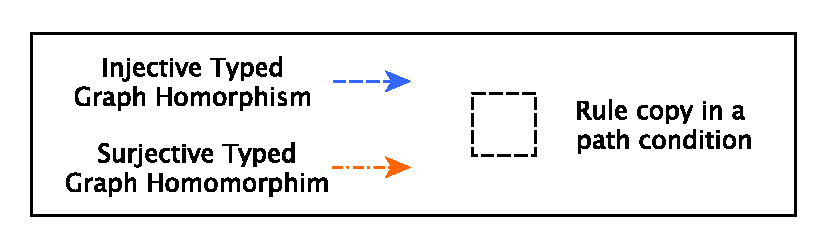
\includegraphics[width=0.5\textwidth]{./figures/abstraction_relation/legend.pdf}
                \caption{Legend for abstraction relation figures}
                \label{fig:legend}
\end{figure}
                
\subsubsection{Example 1 -- Empty Path Condition}

We begin by defining which transformation executions an empty path condition
will abstract. \cref{fig:empty_pc} demonstrates two cases. In each, the path
condition \textit{pc} is on the left-hand side, and a transformation execution \textit{ex} is on the
right-hand side. Note that in \cref{fig:empty_pc_success}, the path condition
abstracts the transformation execution, while in \cref{fig:empty_pc_fail}, the
abstraction relation does not hold.

\begin{figure}[htb]
        \centering
        \begin{subfigure}[b]{0.40\textwidth}
                \centering
                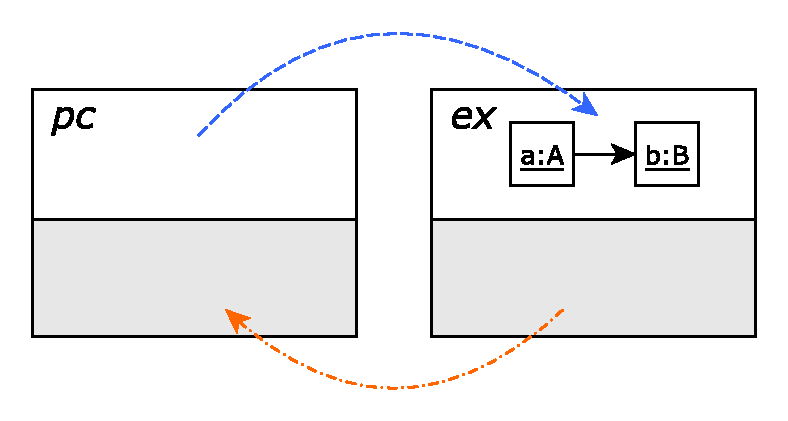
\includegraphics[width=1\textwidth]{./figures/abstraction_relation/empty_pc.pdf}
               	\caption{Abstraction holds}
               	\label{fig:empty_pc_success}
        \end{subfigure}%
        ~~\\
        \begin{subfigure}[b]{0.40\textwidth}
                \centering
                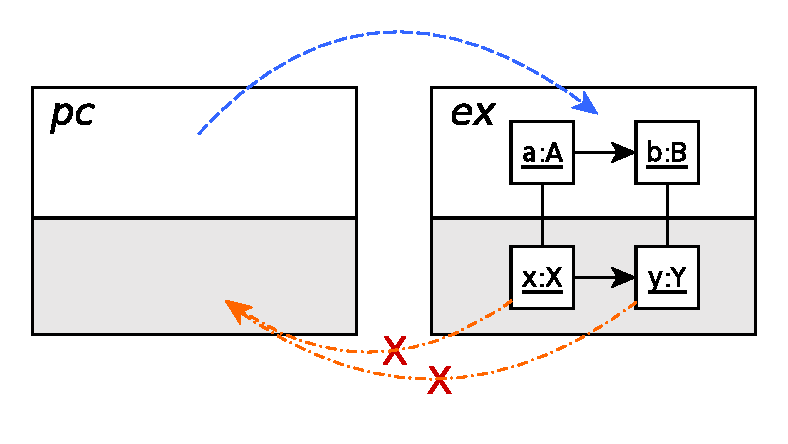
\includegraphics[width=1\textwidth]{./figures/abstraction_relation/empty_pc2.pdf}
                \caption{Abstraction does not hold}
                \label{fig:empty_pc_fail}
        \end{subfigure}%
        \caption{Abstraction of transformation executions by the empty path condition}
        \label{fig:empty_pc}
\end{figure}


The match part of the path condition represents the pre-conditions for the path condition to be true, depending on which rules have symbolically executed in the transformation. For example, if the match graph is empty, this represents all executions where no rules have executed. 

The first condition for the abstraction relation is to determine whether a typed graph injective homomorphism can be found between the match graph of the path condition, and a transformation execution. Note that in both \cref{fig:empty_pc_success} and \cref{fig:empty_pc_fail}, an empty typed graph homomorphism satisfies this condition, highlighted by blue arrows.


The second condition for the abstraction relation is whether a typed graph surjective homomorphism can be found from the transformation execution's output model to the apply graph of the path condition. This is represented by orange arrows in \cref{fig:empty_pc_success} and \cref{fig:empty_pc_fail}. This relation is surjective as there may not be any elements in the output model that are not represented by the path condition's apply graph. Note that multiple elements in the output model may match to the same element in the apply graph of the path condition. This is expected, as the structure found in the apply graph may be found multiple times in the output model.


The empty apply graph of the path condition defines no post-conditions on the output model, as no rules have executed. Note that there an empty surjective typed graph homomorphism can be found between the output model of the transformation execution in \cref{fig:empty_pc_success} and the path condition. This is intuitive, as the lack of elements in the output model means no rules have executed, which corresponds to the lack of post-conditions defined by the path condition.


In contrast, there is no surjection between the elements of the output model in \cref{fig:empty_pc_fail} and the path condition. Note that the transformation execution has elements in the output model and thus at least one rule must have executed. However, the path condition does not represent that a rule has executed. Therefore, the path condition shown does not represent this execution. 

%The fact that this transformation execution will be abstracted by at least one path condition is demonstrated by \cref{prop:pc_completeness}.



\subsubsection{Example 2 -- Non-overlapping Rule Components}


This second example shows the abstraction relation between path conditions and transformation executions, when no match element of the same type appears in multiple rule components.

For these examples, we will represent the abstraction relation with two figures. The first will demonstrate the matching performed on match and apply graphs, while the second figure focuses on traceability link matching.

Let us first examine how the injection operates between the match elements in the path condition and the transformation executions in \cref{fig:non_overlapping_match_apply} and \cref{fig:non_overlapping2_match_apply}. Note that this injection can be found in both cases.

\begin{figure}[htb]
        \centering
        \begin{subfigure}[b]{0.40\textwidth}
                \centering
                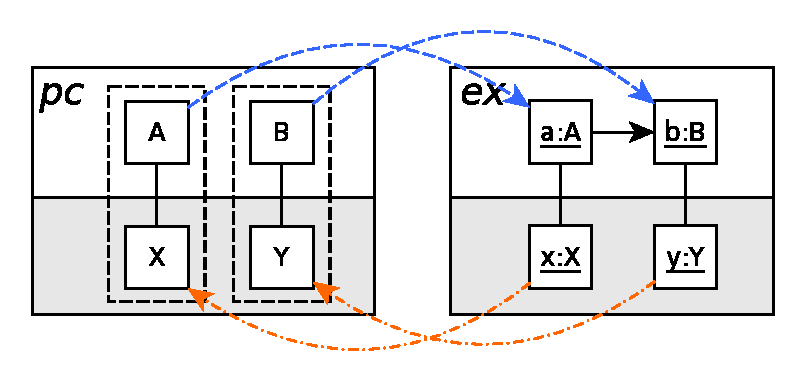
\includegraphics[width=1\textwidth]{./figures/abstraction_relation/non_overlapping.pdf}
               	\caption{Abstraction holds on match and apply graphs}
               	\label{fig:non_overlapping_match_apply}
        \end{subfigure}%
        ~~\\
        \begin{subfigure}[b]{0.40\textwidth}
                \centering
                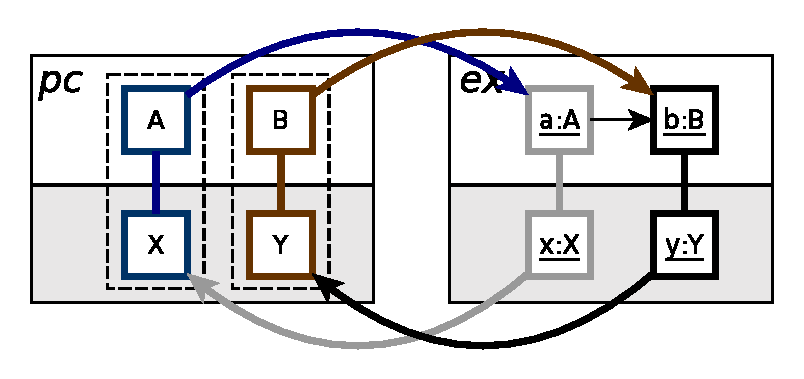
\includegraphics[width=1\textwidth]{./figures/abstraction_relation/non_overlapping_trace_links.pdf}
                \caption{Abstraction holds on traceability links}
                \label{fig:non_overlapping_trace_links}
        \end{subfigure}%
        \caption{Abstraction of transformation execution by non-overlapping rule components}
        \label{fig:non_overlapping}
\end{figure}


\begin{figure}[htb]
        \centering
        \begin{subfigure}[b]{0.40\textwidth}
                \centering
                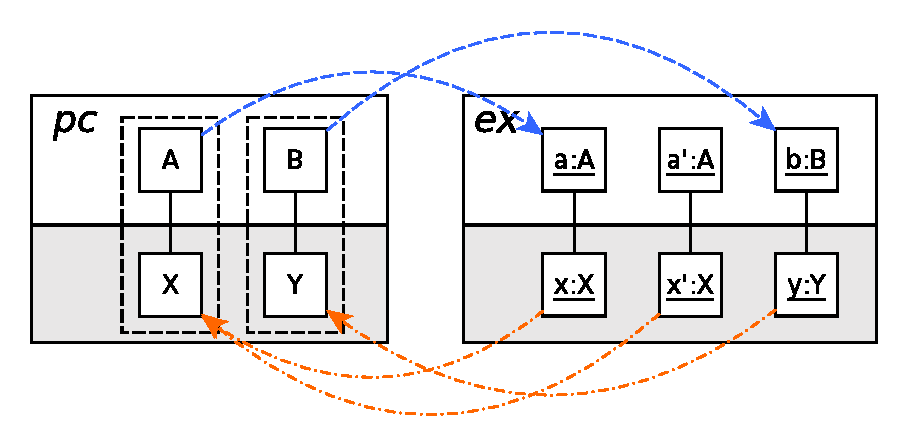
\includegraphics[width=1\textwidth]{./figures/abstraction_relation/non_overlapping2.pdf}
               	\caption{Abstraction holds on match and apply graphs}
               	\label{fig:non_overlapping2_match_apply}
        \end{subfigure}%
        ~~\\
        \begin{subfigure}[b]{0.40\textwidth}
                \centering
                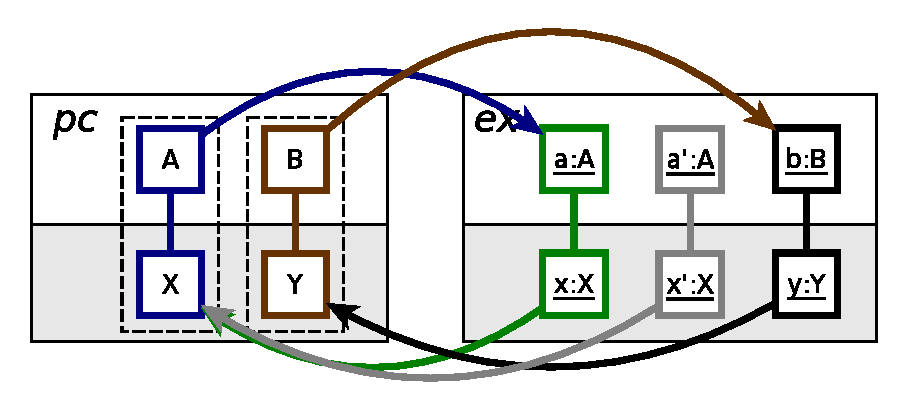
\includegraphics[width=1\textwidth]{./figures/abstraction_relation/non_overlapping2_trace_links.pdf}
                \caption{Abstraction holds on traceability links}
                \label{fig:non_overlapping2_trace_links}
        \end{subfigure}%
        \caption{Example of abstraction over multiple rule execution}
        \label{fig:non_overlapping2}
\end{figure}

Similarly, there is a surjection between the elements of the output model for both transformation execution and the apply graph of the respective path condition. Note that this surjective match also holds in \cref{fig:non_overlapping2_match_apply}, where examination of the transformation execution shows that one rule has executed twice. As mentioned before, the abstraction relation abstracts over the number of times that a rule has executed.

We also note that these matches must also match over associations between the elements, including association typing. This is not included in the figures for visual clarity.


We now examine \cref{fig:non_overlapping_trace_links} and \cref{fig:non_overlapping2_trace_links} to resolve whether the traceability links in the path condition can be found in the transformation execution. This matching is represented by the arrows from each component highlighted in a bold outline and differentiated by colour. We note that each component in the path condition can be successfully found in the transformation execution.

As well, there is a matching step from each individual traceability link in the transformation execution onto the path condition. Similar to the matching from the path condition, the bold components in the transformation execution figure are matched onto the path condition. We note that this matching is successful as well.


\subsubsection{Example 3 -- Overlapping Rule Components}
\label{subsubsec:abstraction_relation_overlapping}

For these examples, the path conditions contain overlapping rule components, i.e. separate rules share match elements of the same type. Our goal is to illustrate the interaction of rule elements, where the elements of non-dependent rules may match over the same or different elements in the transformation execution.

For example, the two rule components in \cref{fig:overlapping_match_apply} correctly match over the transformation execution shown. The abstraction relation holds due to the fact that, while match elements of the same component need to be found injectively in the execution, the injection constraint does not span multiple components. This allows the match elements from different rules to match to the same input model element.


\begin{figure}[htb]
        \centering
        \begin{subfigure}[b]{0.40\textwidth}
                \centering
                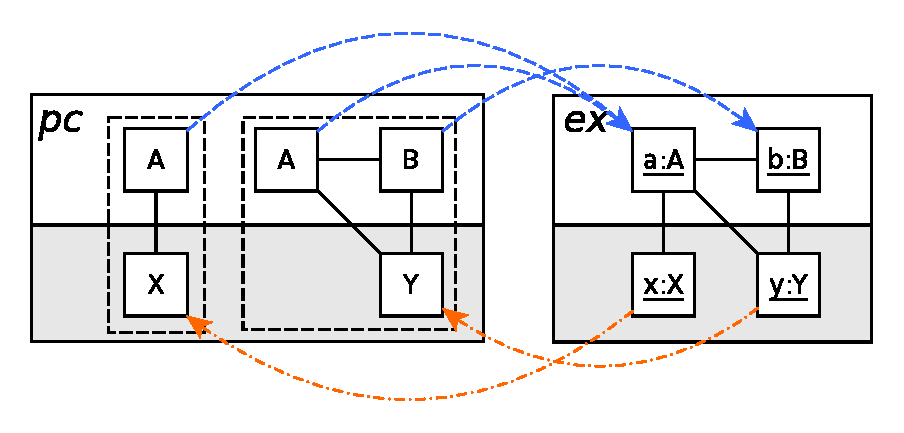
\includegraphics[width=1\textwidth]{./figures/abstraction_relation/overlapping.pdf}
               	\caption{Abstraction holds on match and apply graphs}
               	\label{fig:overlapping_match_apply}
        \end{subfigure}%
        ~~\\
        \begin{subfigure}[b]{0.40\textwidth}
                \centering
                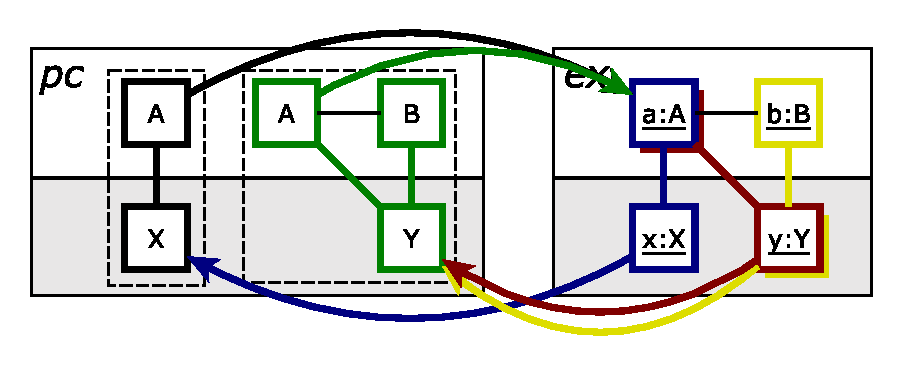
\includegraphics[width=1\textwidth]{./figures/abstraction_relation/overlapping_trace_links.pdf}
                \caption{Abstraction holds on traceability links}
                \label{fig:overlapping_trace_links}
        \end{subfigure}%
        \caption{Abstraction of transformation execution by overlapping rule components}
        \label{fig:overlapping}
\end{figure}

As well, \cref{fig:overlapping_trace_links} shows the mapping from the path condition to the transformation execution. However, note that the pattern composed of the A, B, and Y elements, along with the traceability links, is to be matched as a whole. This is to ensure that the traceability links are found in the proper configuration in the transformation execution.

We also match the traceability links from the transformation execution back onto the path condition. Again, this is to ensure that no traceability links are found in the transformation execution that have not been represented in the path condition. Three matches are performed in this step, denoted by the three arrows in the bottom of \cref{fig:overlapping_trace_links}. Each match is composed of a traceability link as well as immediately connected elements.

\begin{figure}[htb]
        \centering
        \begin{subfigure}[b]{0.40\textwidth}
                \centering
                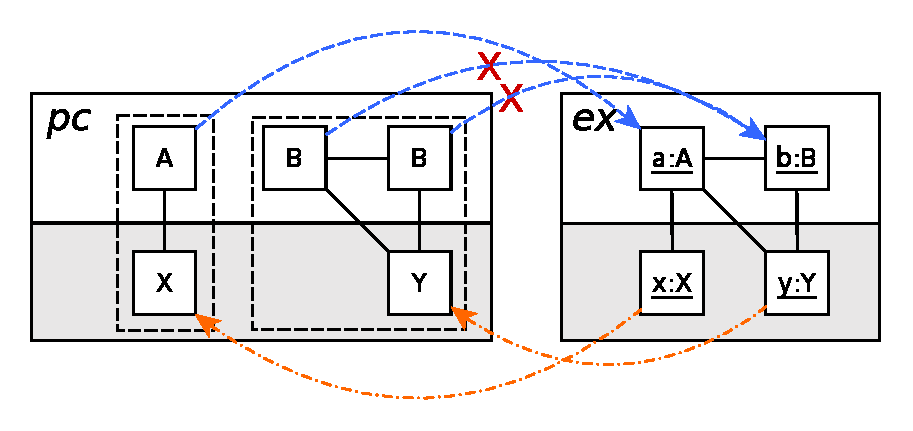
\includegraphics[width=1\textwidth]{./figures/abstraction_relation/overlapping2.pdf}
               	\caption{Elements cannot overlap within a component}
               	\label{fig:overlapping2_match_apply}
        \end{subfigure}%
        ~~\\
        \begin{subfigure}[b]{0.40\textwidth}
                \centering
                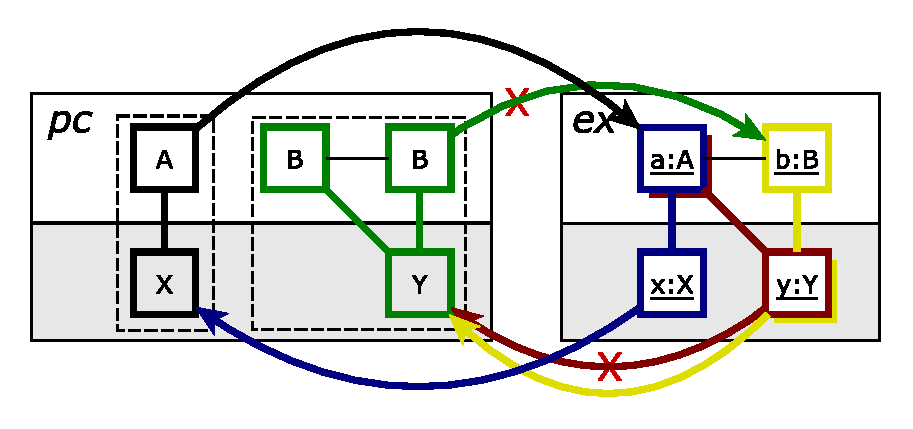
\includegraphics[width=1\textwidth]{./figures/abstraction_relation/overlapping2_trace_links.pdf}
                \caption{Traceability links cannot be found}
                \label{fig:overlapping2_trace_links}
        \end{subfigure}%
        \caption{Abstraction does not hold}
        \label{fig:overlapping2}
\end{figure}


In contrast to \cref{fig:overlapping}, \cref{fig:overlapping2} shows an example where the abstraction relation does not hold. Consider \cref{fig:overlapping2_match_apply}. Note that a component in the match graph of the path condition contains two B elements. Both of these elements must be found in the transformation execution, and thus it is not correct for them to injectively match to the same element in the input model.

As well, it is informative to examine \cref{fig:overlapping2_trace_links}. Note the one of the matches from the transformation execution attempts to match over 'a:A' and 'y:Y' elements, connected by a traceability link. Examination of the path condition shows that this traceability link is not present. Therefore, this path condition cannot accurately represent this transformation execution.


\subsubsection{Example 4 -- Indirect Links}

\begin{figure}[htb]
        \centering
        \begin{subfigure}[b]{0.40\textwidth}
                \centering
                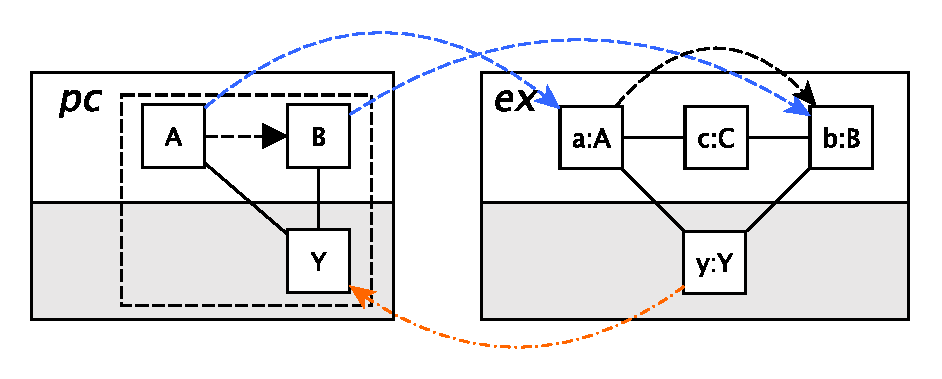
\includegraphics[width=1\textwidth]{./figures/abstraction_relation/indirect.pdf}
               	\caption{Matching over match and apply graphs}
               	\label{fig:indirect_match_apply}
        \end{subfigure}%
        ~~\\
        \begin{subfigure}[b]{0.40\textwidth}
                \centering
                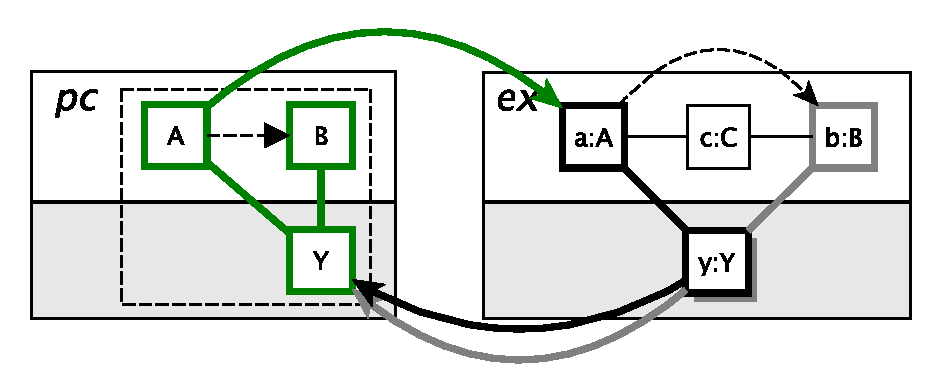
\includegraphics[width=1\textwidth]{./figures/abstraction_relation/indirect_trace_links.pdf}
                \caption{Matching over traceability links}
                \label{fig:indirect_trace_links}
        \end{subfigure}%
        \caption{Abstraction with indirect links}
        \label{fig:indirect}
\end{figure}

\begin{figure*}[htb]
        \centering
        \begin{subfigure}[b]{0.70\textwidth}
                \centering
                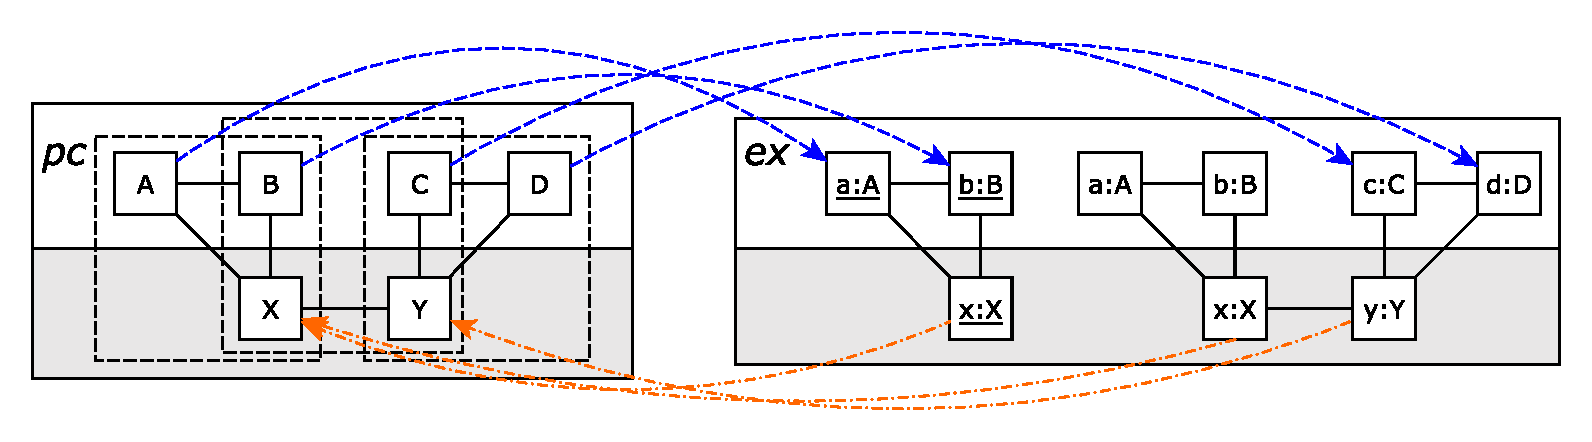
\includegraphics[width=1\textwidth]{./figures/abstraction_relation/combination.pdf}
               	\caption{Abstraction holds on match and apply graphs}
               	\label{fig:combination_match_apply}
        \end{subfigure}%
        ~~\\
        \begin{subfigure}[b]{0.70\textwidth}
                \centering
                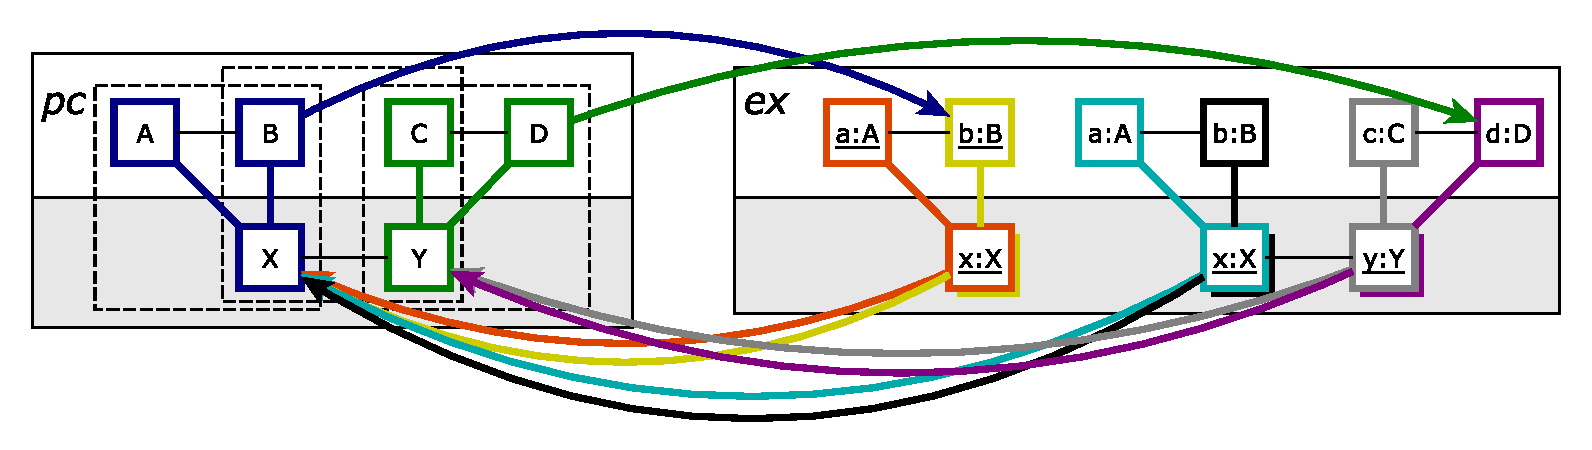
\includegraphics[width=1\textwidth]{./figures/abstraction_relation/combination_trace_links.pdf}
                \caption{Abstraction holds on traceability links}
                \label{fig:combination_trace_links}
        \end{subfigure}%
        \caption{Abstraction where path condition has combined rules}
        \label{fig:combination}
\end{figure*}

We now present a path condition  in \cref{fig:indirect_match_apply} that includes indirect links. In this case, for the injective match to hold, the elements at both ends of the link must be found, and there must be an indirect link between the matched elements and between the elements in the transformation execution.

Note that the indirect link between elements $a:A$ and $b:B$ in the transformation execution is added by the containment transitive closure $Input^{*}$ in proposition~\ref{eq:abstr_input_output} of \cref{def:abstraction_pc_ex} to allow matching indirect links. Note also that, for the sake of our example, we are assuming that the links between $a:A$, $b:b$ and $c:C$ are containment relations.

\cref{fig:indirect_trace_links} highlights the structures involved in matching over traceability links. From the path condition, the structure contains the A, B, and Y elements with connected traceability links. From the transformation execution, there are two structures to be found in the path condition denoted in bold in the transformation execution. The matching of all structures can be successfully performed, and thus this abstraction relation holds.


%Note that only the match graph of the path condition may include an indirect link.



\subsubsection{Example 5 -- Combined Rules}



\cref{fig:combination} shows a path condition that is composed of a multitude of rules which have been combined in the path condition generation algorithm. Each individual rule is surrounded by dashed lines.

Note that the matching on the match and apply graphs in \cref{fig:combination_match_apply} is similar to other examples. The combined rules can be considered as a single graph for the abstraction relation.

\cref{fig:combination_trace_links} shows the matching when multiple traceability links are present in the transformation execution. Note that each individual traceability link and the connected elements are matched onto the path condition.

